\documentclass{article}
\usepackage[utf8]{inputenc}
\usepackage[hidelinks]{hyperref}
\usepackage[spanish]{babel}
\usepackage[left=2cm,right=2cm,top=2cm,bottom=2cm]{geometry}
\usepackage{graphicx}
\usepackage{pdflscape}
\usepackage{listings}

\lstset {
    frame = single,
    breaklines = true
}

\begin{document}

\begin{titlepage}
\title{\textbf{\Huge{Práctica 1: Diseño e Implementación de un \textit{Data Mart}}\\
\large{Almacenes y Minería de Datos}}}
\author{
    Pedro Allué Tamargo (758267)
    \and
    Cristina Oriol García (755922)
    \and
    Alejandro Paricio García (761783)
}

\date{\today}
\clearpage\maketitle
\thispagestyle{empty}
\end{titlepage}

% Indice
\tableofcontents

\newpage
\section{Data Mart para vuelos comerciales}
\subsection{Metodología de \textit{Kimball} aplicada, diseño del \textit{Data Mart}}

Siguiendo la metodología de \textit{Kimball} se va a diseñar un \textit{Data Mart} para el análisis de la información de vuelos comerciales en Estados Unidos.\\
El primer paso en esta metodología consiste en la selección del proceso de negocio. En este caso el proceso de negocio se va a centrar en el estudio del tiempo total de los vuelos y sus retardos (si estos existiesen). Se estudiarán factores asociados a los vuelos como los aeropuertos de origen, destino y que días existe un peor rendimiento. Este \textit{Data Mart} se centrará en los usuarios que tienen cabida en el proceso de toma de decisiones en el ámbito de la aviación comercial.\\

El siguiente paso es la elección del gránulo o nivel detalle de los datos. Se ha elegido un vuelo de un avión determinado en una fecha y horas de salida concretas. Utilizando e grano más fino posible conseguiremos que se centre en la información indivisible generada por el proceso de negocio para poder tener la flexibilidad necesaria para formular cualquier pregunta.\\

El tercer paso es la elección de las dimensiones primarias y secundarias. Las dimensiones primarias son las que son determinadas por el grano escogido para los hechos, por lo que, obviamente, van a ser Fecha (de salida), Hora (de salida), Avión. Un vuelo va a poderse identificar mediante su fecha y hora de salida y el avión encargado de realizar el vuelo en cuestión.\\
El resto de dimensiones van a ser secundarias y, por definición, tomarán un único valor por combinación de las dimensiones primarias. No aportan información directa acerca de la identificación del hecho ``vuelo'', y no formarán parte de la clave primaria de la tabla de hechos. Conforman este conjunto las dimensiones Aeropuerto (de origen y de destino), Operadora, Aerolínea, Fecha (de llegada), Hora (de llegada).\\

En el último de los pasos ha de refinarse qué se está midiendo e identificarse que hechos numéricos poblarán cada tupla de la tabla de hechos. Finalmente, se han incluido como hechos numéricos en la tabla de hechos ``Vuelo'' los siguientes:

\begin{itemize}
    \item Tiempo real de Vuelo = hora de llegada real - hora de salida real. (minutos)
    \item Tiempo estimado de vuelo = hora de llegada estimada - hora salida estimada. (minutos)
    \item Tiempo de Retraso a la llegada = máximo entre la diferencia de la hora de llegada real y la hora de salida estimada y 0. (minutos)
    \item Tiempo total de vuelo = Hora de llegada real - hora de salida estimada. (minutos)
    \item Tiempo de retraso a la salida = Hora de salida real - hora de salida estimada. (minutos)
    \item Tiempo adelantado a la llegada = máximo entre la diferencia de la hora de llegada estimada y la hora de llegada real y 0. (minutos)
\end{itemize}

Entre los aspectos que dieron lugar a debate en el proceso anterior encontramos:
\begin{itemize}
    \item El identificador del vuelo (\textit{numeroVuelo}) es un número que se asigna en función de la aerolínea y la fecha \cite{wiki:1}. Ello ha condicionado el no poder ser utilizada para determinar el avión de un vuelo determinado de manera unívoca, y por tanto no es una clave natural. Si que aparece como una clave natural el atributo matriculaAvion, que si es único para cada avión.
    \item La separación de las dimensiones Fecha y Hora es motivada por la posibilidad de que aparezca una explosión combinatoria. Por ejemplo, para 365 días y 24 horas al día, una única tabla podría llevar a un máximo de 365*24 tuplas, mientras que con dos, queda limitado a 365+24 tuplas.
    \item Finalmente, se ha considerado el \textit{numeroVuelo} como una dimensión degenerada (\textit{DD}), ya que correspondería a una dimensión secundaria adicional. Contiene información que puede llegar a ser relevante, pero no puede ser tratada como las demás ya que no contiene más atributos que el propio \textit{númeroVuelo} y por lo tanto se corresponde con una dimensión degenerada (\textit{DD}).
\end{itemize}

Por lo tanto, teniendo en cuenta todo lo anterior se ha creado el esquema en estrella de la Figura \ref{fig:esquema_estrella_1}.

\subsection{Alternativas consideradas}

Una de las alternativas en el diseño del \textit{data mart} que se consideraron atañe a las dimensiones con múltiples conexiones a la tabla de hechos en el esquema original. Motivados por aportar facilidad a los usuarios, que a la hora de llevar a cabo consultas que aprovechen ambas relaciones deberán renombrar la tabla de varias formas, se podría llevar a cabo la siguiente modificación, dividiendo conceptualmente la dimensión fecha en \textit{FechaSalida} y \textit{FechaLlegada} (cambio repetido no sólo para esa tabla, sino también para Hora y Aeropuerto).

\begin{figure}[hbpt]
    \centering
    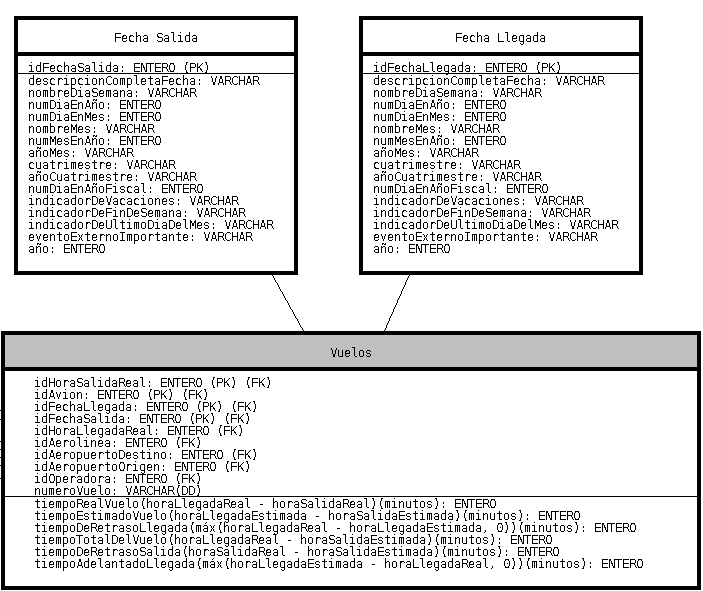
\includegraphics[scale=0.4]{images/fechas.png}
    \caption{Modificaciones al esquema en estrella}
    \label{fig:esquema_estrella_opcional}
\end{figure}

A la hora de implementar el esquema, se llevaría a cabo como única tabla física sobre la que se definirían dos vistas, denominadas \textit{FechaSalida} y \textit{FechaLlegada}.\\
Como ejemplo ilustrativo del aporte que puede suponer a los usuarios, se despliega parte de una consulta que lo refleje:

\begin{itemize}
    \item Implementación original: FROM Fecha AS FechaSalida, Fecha AS FechaOrigen.
    \item Implementación alternativa: FROM FechaSalida, FechaOrigen
\end{itemize}

Pese a ser una alternativa a valorar, se ha considerado que al haber un máximo de dos relaciones de una tabla de dimensión cualquiera a la tabla de hechos, no va a resultar problema alguno para el usuario el no disponer de las dos vistas, y que puede prescindirse de lo anterior.

\subsection{Aspectos de implementación del esquema en estrella \textit{SQL} y del poblado}

Para generar el código \textit{SQL} de este diagrama en estrella se va a utilizar la funcionalidad de la herramienta \textit{DBDap} que extrae el \textit{SQL} a partir del esquema en estrella. Se ha observado que una vez generado este código no se reconoce el tipo \textit{VARCHAR} y se genera como \textit{CHAR(-1)}. También se ha tenido que añadir manualmente las restricciones de \textit{NOT NULL} a los atributos. Dando como resultado al código al código \ref{list:codigo_tablas_1}. Conjuntamente al script de creación se ha creado el de borrado de tablas.\\

Para crear los datos de población del almacén de datos se ha creado un \textit{script Python} (código \ref{list:codigo_poblar}) que crease las sentencias de inserción \textit{SQL} a partir de un conjunto de datos de aeropuertos, aviones, aerolíneas y operadoras.\\


\section{Modificación del \textit{Data Mart} de vuelos comerciales}

Para este apartado se ha modificado el esquema en estrella del apartado anterior (Figura \ref{fig:esquema_estrella_1}) para reflejar la información de los asientos. Originalmente se planteó como idea modificar el gránulo, ya que este no coincidía con el nivel de detalle de los asientos. No obstante, al incluir redundancia innecesaria sin aportar grandes ventajas para el análisis (necesitarías tener el tiempo de vuelo para cada asiento, que coincidiría con el del resto de asientos del vuelo, y no aportaría nada al análisis de los retardos y rendimiento), terminó descartándose. Se debía buscar otra solución, y se optó por las dimensiones puente (\textit{bridge dimensions}) \cite{nuwa:1}.\\

Una primera aproximación que se pensó fue guardar la información del asiento con la de los pasajeros. No obstante, el asiento no es único para todos los vuelos que realiza ese avión. Por lo tanto, se decidió utilizar el pasajero (ya que es lo que se pide almacenar) y la información del asiento se guardará con la información del anterior.\\

Se ha creado el esquema en estrella de la Figura \ref{fig:esquema_estrella_asiento} en el cual se puede observar que la tabla de hechos sigue siendo ``vuelo'' y que tiene una conexión con la tabla de dimensiones \textit{Pasajeros Vuelo Bridge}. Esto implica que cada vuelo está conectado con la dimensión puente que relaciona el vuelo con el pasajero que ocupa un asiento en el mismo. La dimensión \textit{Pasajero} está conectada con esta dimensión puente ya que todos los pasajeros pertenecen a un vuelo.\\

Para la generación del esquema \textit{SQL} se ha utilizado de nuevo las opciones proporcionadas por \textit{DBDap} La diferencia con respecto al apartado anterior ha sido la generación de dos tablas extra correspondientes a las nuevas dimensiones.\\

Con respecto a la introducción de datos de este esquema se han añadido manualmente los datos de las tablas nuevas sobre los datos de población generados por el \textit{script} (código \ref{list:codigo_poblar}) del apartado anterior. El código \textit{SQL} de creación de tablas se puede observar en el código \ref{list:codigo_tablas_2}. \\

\newpage
\section{Enunciado propuesto: Alquiler de coches en Europa}

Se desea implantar un \textit{data mart} para el análisis de información de alquiler de vehículos de una empresa con sucursales por Europa. Se quiere almacenar los siguientes datos de cada alquiler: sucursal de recogida y de depósito del vehículo (\textit{nombre}, \textit{código} y \textit{dirección}), país de origen y destino, ciudad de origen y destino, modelo del vehículo (\textit{marca}, \textit{nombre}, \textit{matrícula}) y la fecha de la recogida y la devolución del vehículo. Además de los anteriores, se desea guardar la fianza exigida al cliente y el seguro adquirido, el nombre de la compañía aseguradora, así como el límite económico del que se hace responsable la empresa y el importe del mismo, además del precio y el tiempo del alquiler (se alquilará por días) y las características del cliente (\textit{nombre}, \textit{edad}, \textit{estado civil}, \textit{género}, \textit{situación laboral}).\\

El análisis se va a centrar en el rendimiento económico de los alquileres y el beneficio o pérdida obtenidos. Se desea saber con qué coches se obtiene un mayor beneficio y que tipo de clientes lo proporcionan, así como cuáles son los seguros cuya contratación más dinero reporta.\\

El grano se va a definir como un alquiler en una fecha de recogida de un vehículo determinado por parte de un cliente en una sucursal concreta. Ello va a dar lugar al esquema de la Figura \ref{fig:esquema_estrella_alquiler}.\\

En el diagrama en estrella desarrollado se puede observar que las dimensiones primarias son: Sucursal (Origen), Vehículo, Cliente y Fecha (recogida del vehículo en la sucursal de origen), es decir, aquellas que definen el grano.\\

En la tabla de hechos \textit{Alquiler} se puede observar que se han añadido los atributos correspondientes para el estudio del rendimiento económico de las sucursales de alquiler de vehículos. Los atributos que se van a estudiar son:

\begin{itemize}
    \item Días de duración del alquiler (días).
    \item Importe cargado al cliente. Sin tener en cuenta el importe de la fianza y teniendo en cuenta el importe del seguro (euros).
    \item Gasto de la empresa. Gasto al que hace frente la empresa de alquiler por motivos como el mantenimiento del vehículo, limpieza... (euros)
    \item Beneficio sin descontar impuestos. Beneficio bruto obtenido del importe cargado al usuario y los gastos de la empresa (euros).
    \item Beneficio descontando impuestos. Beneficio de la empresa tras aplicar impuestos (euros).
    \item Fianza. Importe abonado por el cliente (euros).
    \item Importe de seguro abonado por el cliente (euros). 
\end{itemize}

De nuevo, se podría considerar aplicar la misma alternativa propuesta para el primer apartado de la práctica, lo que podría variar ligeramente la implementación del modelo.

\newpage
\section{Conclusiones}

En esta práctica se ha hecho una primera aproximación a los almacenes de datos. Se han creado esquemas en estrella siguiendo la metodología de \textit{Kimball} a partir de una breve descripción del problema. Se ha determinado el proceso de negocio para la creación de este \textit{Data Mart} y se ha seleccionado el gránulo adecuado. Además, se han elegido las dimensiones de manera consecuente a las decisiones tomadas en los pasos anteriores y se ha plasmado el esquema conceptual mediante el uso de la herramienta \textit{DBDap}. Por último, se ha traducido ese esquema a una implementación correcta y coherente, siendo valoradas distintas alternativas y corrigiéndose los errores derivados de la automatización del proceso de generar código \textit{SQL}. Todo el proceso ha sido llevado a cambo habiendo analizado y teniendo en cuenta las necesidades de los usuarios.\\

La metodología de \textit{Kimball} es un proceso que sigue 4 etapas para el diseño de \textit{Data Mart}. Siguiendo esta metodología y pensando en el usuario final que deberá utilizar este sistema se han diseñado de una forma eficiente los \textit{Data Marts} de esta práctica.
EL único gran problema observado con este \textit{Data Mart} y el procedimiento utilizado para su construcción atañe a la relación de este con futuras prácticas. En lugar de diseñar el esquema global y, tras ello, centrarnos en cada uno de los esquemas individuales a cada proceso de negocio, se ha acudido directamente al segundo. Esto puede llegar a crear mucho conflictos si es necesario integrarlo con los creados en futuras prácticas ya que pueden existir problemas con la integración tipos de datos y con dimensiones que deban estar conformados.\\

\subsection{Control de esfuerzos}

El trabajo se ha realizado en su parte mayoritaria en la sesión de prácticas. Se han concretado varias reuniones entre los integrantes del grupo, una antes de la sesión de prácticas y un dos después de la misma para poner en común el trabajo realizado por cada uno y ofrecer alternativas e ideas. Las herramientas utilizadas para la práctica han sido \textit{DBDap}, \textit{dBeaver} como herramienta de conexión a bases de datos y, finalmente, \textit{Python} para la generación de los \textit{scripts} necesarios. Cada uno de los integrantes han realizado los siguientes trabajos:

\begin{itemize}
    \item Pedro Allué Tamargo: creación del esquema en estrella de vuelos, creación del esquema en estrella de alquileres de coches, redacción de la memoria. Tiempo invertido: 10 horas.
    \item Cristina Oriol García: creación del esquema en estrella de vuelos, creación del esquema en estrella de alquileres de coches, creación del esquema en estrella de vuelos contemplando los asientos, poblar almacén de datos de vuelos con asientos. Tiempo invertido: 11 horas.
    \item Alejandro Paricio García: creación del esquema en estrella de vuelos, creación del esquema en estrella de alquileres de coches, poblar almacén de datos de vuelos. Tiempo invertido: 13 horas.
\end{itemize}


\newpage
\begin{landscape}
\section{Anexo 1: Figuras}
\begin{figure}[h!]
    \centering
    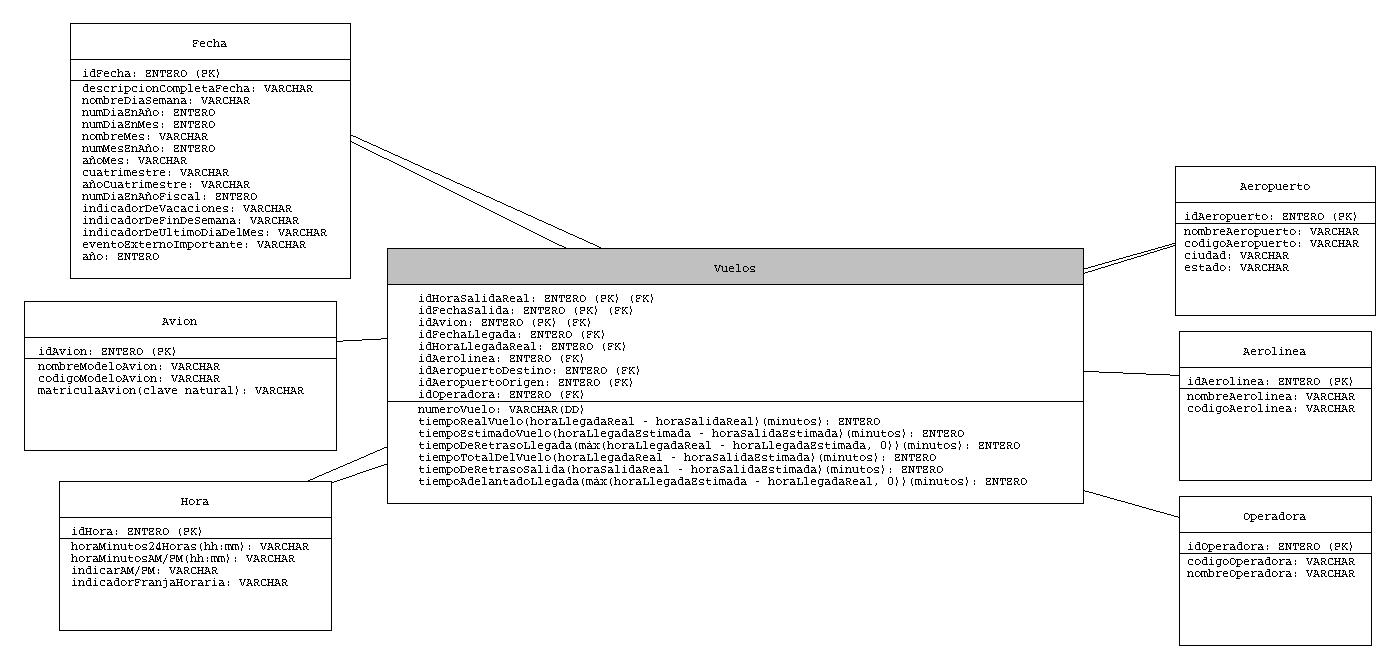
\includegraphics[scale = 0.4]{images/esquema_estrella_1.jpg}
    \caption{Esquema en estrella del \textit{Data Mart} de vuelos comerciales}
    \label{fig:esquema_estrella_1}
\end{figure}
\end{landscape}

\newpage
\begin{landscape}
\begin{figure}
    \centering
    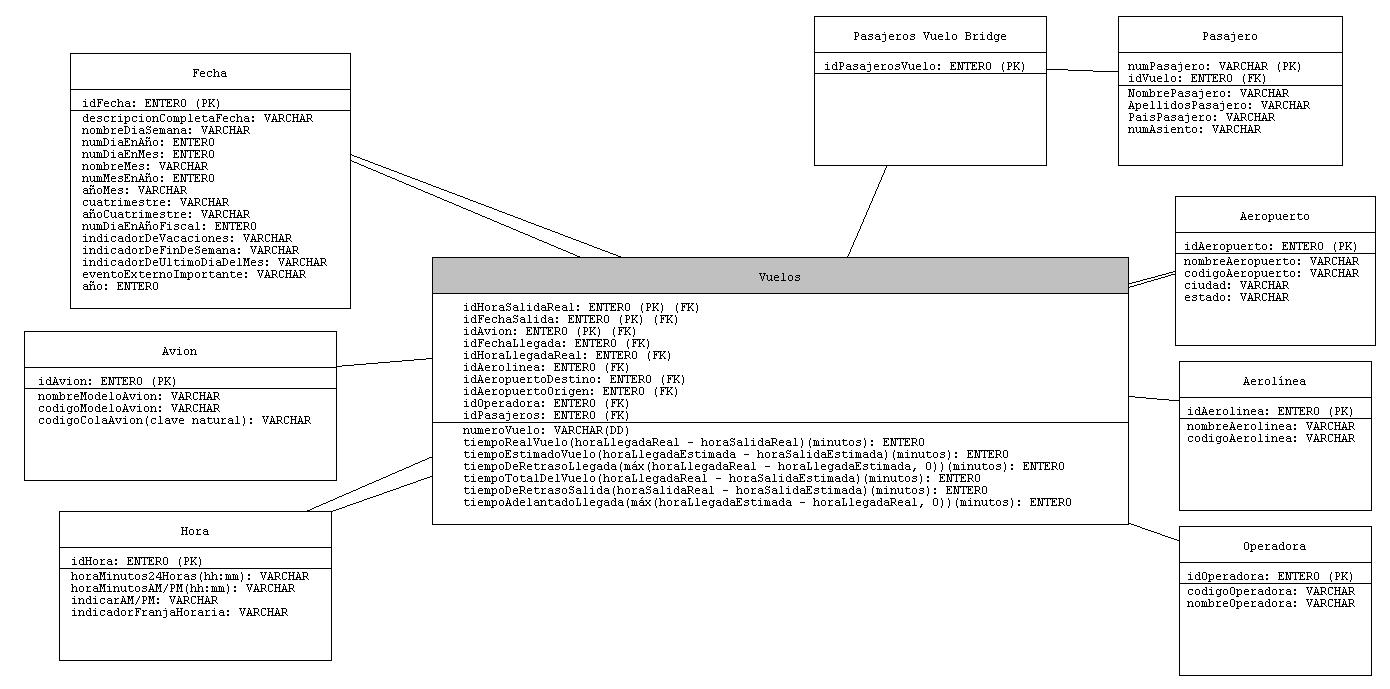
\includegraphics[scale=0.4]{images/p2_2.jpg}
    \caption{Esquema en estrella del \textit{Data Mart} de vuelos comerciales teniendo en cuenta el asiento}
    \label{fig:esquema_estrella_asiento}
\end{figure}
\end{landscape}

\newpage
\begin{landscape}
\begin{figure}[h!]
    \centering
    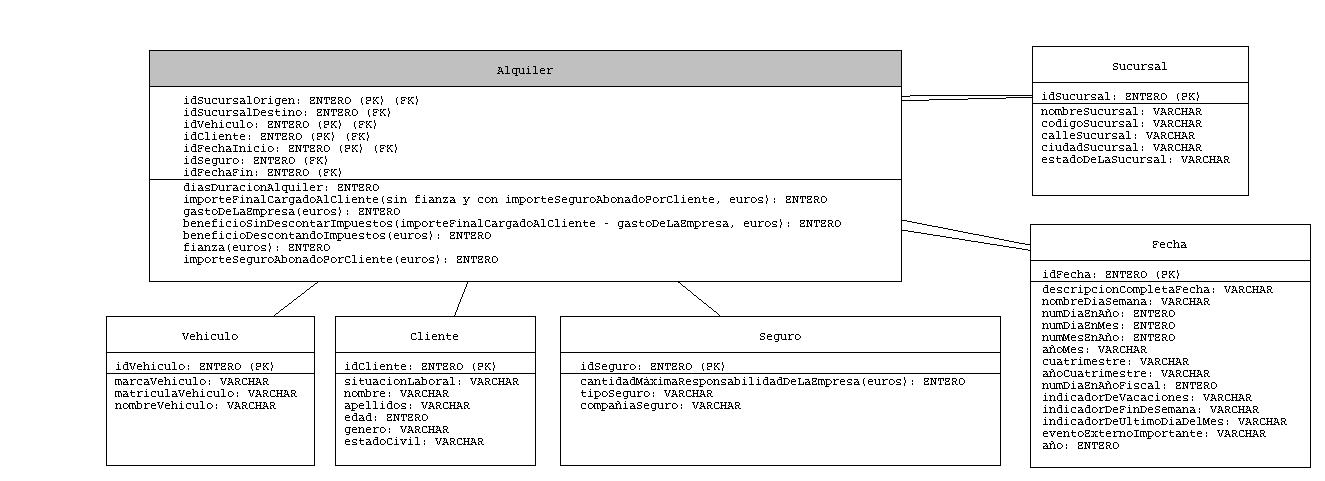
\includegraphics[scale=0.4]{images/esquema_estrella_alquiler.jpg}
    \caption{Esquema en estrella del enunciado propuesto}
    \label{fig:esquema_estrella_alquiler}
\end{figure}
\end{landscape}

\section{Anexo 2: Códigos}

\subsection{Script \textit{SQL} para la creación de las tablas del apartado 1}
\lstinputlisting[label={list:codigo_tablas_1}]{listings/creacionTablas.sql}

\newpage
\subsection{Script \textit{SQL} para la creación de las tablas del apartado 2}
\lstinputlisting[label={list:codigo_tablas_2}]{listings/creadotablasApartado2.sql}

\newpage
\subsection{Script de creación de elementos a insertar \textit{Data Mart} de vuelos comerciales}
\lstinputlisting[label={list:codigo_poblar}]{listings/scriptQueCreaPoblar.py}


\newpage
\addcontentsline{toc}{section}{Referencias}
\bibliographystyle{unsrt}
\bibliography{bibliografia.bib}


\end{document}
